\documentclass[t]{beamer}
%\usepackage{multimedia}		% for movies, sounds, animations...
\usepackage[ngerman]{babel}		% new german
\usepackage[utf8]{inputenc}		% input...

\usepackage{tabularx}			% local, only for this doc.

\usepackage[uniWZ, blockBG, tams, secNum, secToc, blockRound, engl]{tamsBeamer}
%-----------------------------------------------------------------------------
%-- options		------------------------------------------------------
%			tams	|	- TAMS		publication
%			cinacs		- CINACS	publication
%			engl		- english strings	[german]
%			uniWZ	|	- uni		watermark
%			tamsWZ	|	- tams+uni	watermark
%			cinacsWZ	- cinacs+uni	watermark
%			secToc	|	- toc repetition at each section
%			secTocA		- -"-, all sections: show
%					  replacement for toc in short docs
%			subsecToc	- toc repetition at each subsection
%			secNum  	- (sub)-section numbering
%			fullstep	- always step through items
%			noFoot		- footline	off
%			noPage		- page numbers	off
%			noAuth		- author	off
%			conference	- footline with \foottitle{...}
%			blockBG	|	- block, example etc. background
%			blockRound	- -"-, rounded+shadow


% fonts definitions			--------------------------------------
% ----------------------------------------------------------------------------
% default: cmss, OT1 fontenc		good with UniHH font "The Sans"
%					-> don't change fonts!
%\usepackage{times}			% other fonts
%\usepackage[T1]{fontenc}		%

% document definitions			--------------------------------------
% ----------------------------------------------------------------------------
\title[Jaco Arm ROS]			% title		-- option: short
  {Kinova Jaco Arm Control via ROS}
\subtitle[Robot-Era]			% subtitle	-- option: short
  {Robot-Era Project}

\author[J. Liebrecht, S. Rockel]{Johannes Liebrecht\and Sebastian Rockel}

%\author[AutorA, AutorB]		% author	-- option: short
% {A.~Autor\inst{1} \and B.~Autor\inst{2}}%		-- option: \inst{...}
% style option: [tams] predefines institute...
% or define \institute{...}
%					% \inst{...} for different institutions
%\institute[Universities A and B]	% institution	-- option: short
%{ \inst{1}%
%  University of A\\
%  Department of A
%  \and
%  \inst{2}%
%  University of B\\
%  Department of B}

\date[19-nov-2012]			% event/date	-- option: short
  {19.~November 2012}

\subject{TAMS, LaTeX, Folien}		% subject	-- option for pdf


% document starts here			--------------------------------------
% ----------------------------------------------------------------------------
\begin{document}

% titlepage				--------------------------------------
%\frame[plain]{\titlepage}		% suppress head- and footlines
\frame{\titlepage}

% toc					--------------------------------------
 
\begin{frame}
  \frametitle{\tocName}
  \tableofcontents
  %\tableofcontents[pausesections]	% step through sections
\end{frame}

\section{Kinova Jaco Arm Overview}

\frame{\frametitle{Kinova Jaco Arm}
\begin{itemize}
\item 6 degrees of freedom
\item carbon fiber structure
\item total weight: 5Kg
\item reach : 90cm
\end{itemize} 

\begin{figure}
\centering
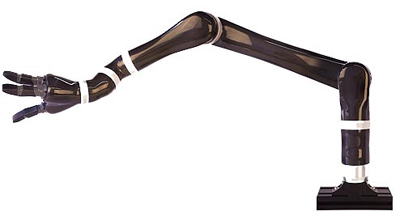
\includegraphics[width=7cm]{kinova2.jpg}
\end{figure}

}

\frame{\frametitle{Kinova Jaco Arm}
\begin{itemize} 
\item Maximum Load : 1.5kg at mid-range/1.0kg at end-range
\item Maximum linear arm speed : 15cm/sec
\item 3 fingers or 2 fingers utilization
\item Finger force limited to 7N 
\end{itemize} 

\begin{figure}
\centering
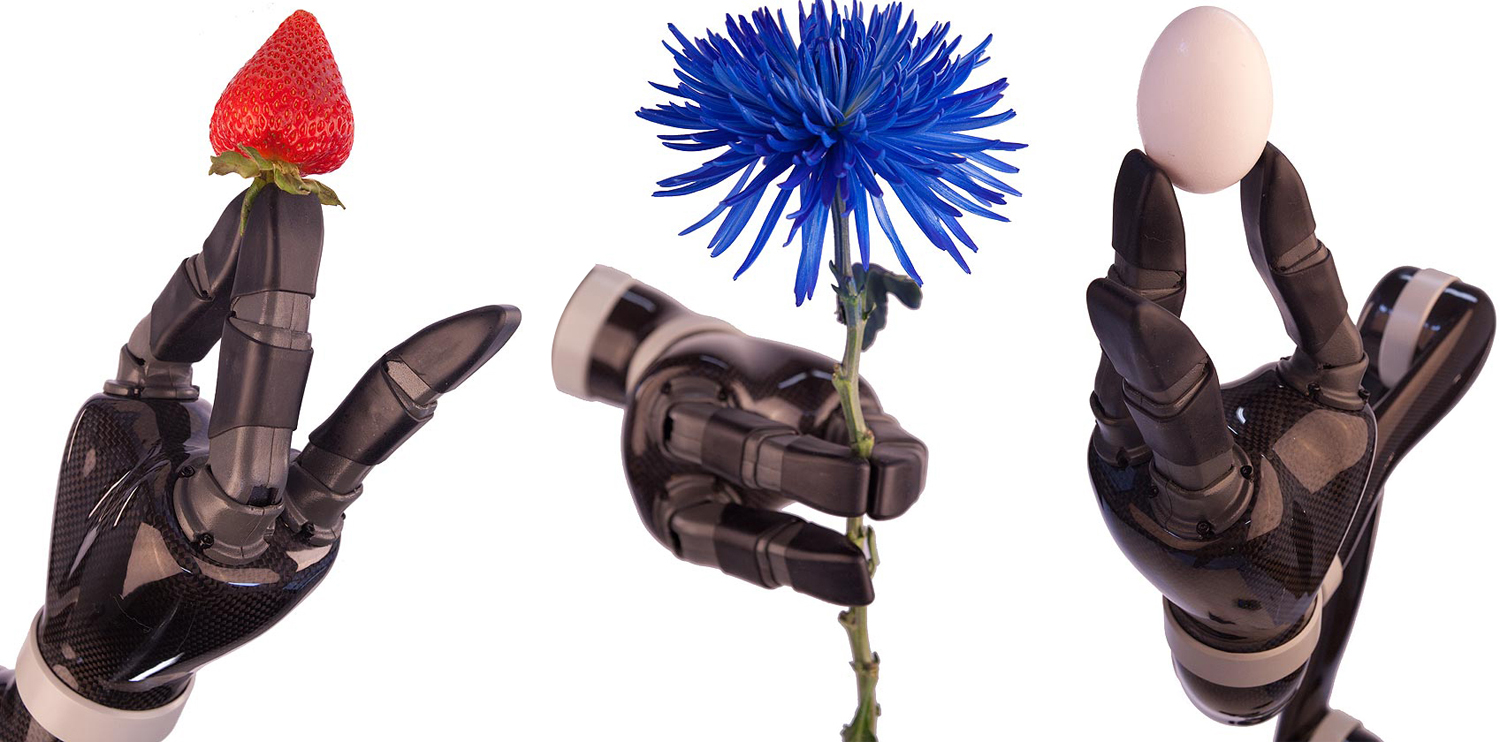
\includegraphics[width=7cm]{kinova.jpg}
\end{figure}

}

 
\frame{\frametitle{Jaco Arm Rest Time}
\begin{figure}
\centering
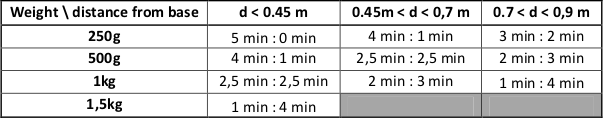
\includegraphics[width=\linewidth]{resttime.png}
\end{figure}
}

\frame{\frametitle{Working with Kinova Jaco Arm}
\begin{itemize} 
\item be aware of collusion with camera head 
\item home position/ retract position
\end{itemize} 
}   

\section{Kinova Jaco Arm Library}

\frame{\frametitle{Jaco Arm Library}
\begin{itemize} 
\item powerful library(C\#)
\item documentation (\url{Jaco_API} Programming Guide)
\item view dynamic-link library with MonoDevelop
\end{itemize} 
}

\frame{\frametitle{MonoDevelop}
\begin{figure}
\centering
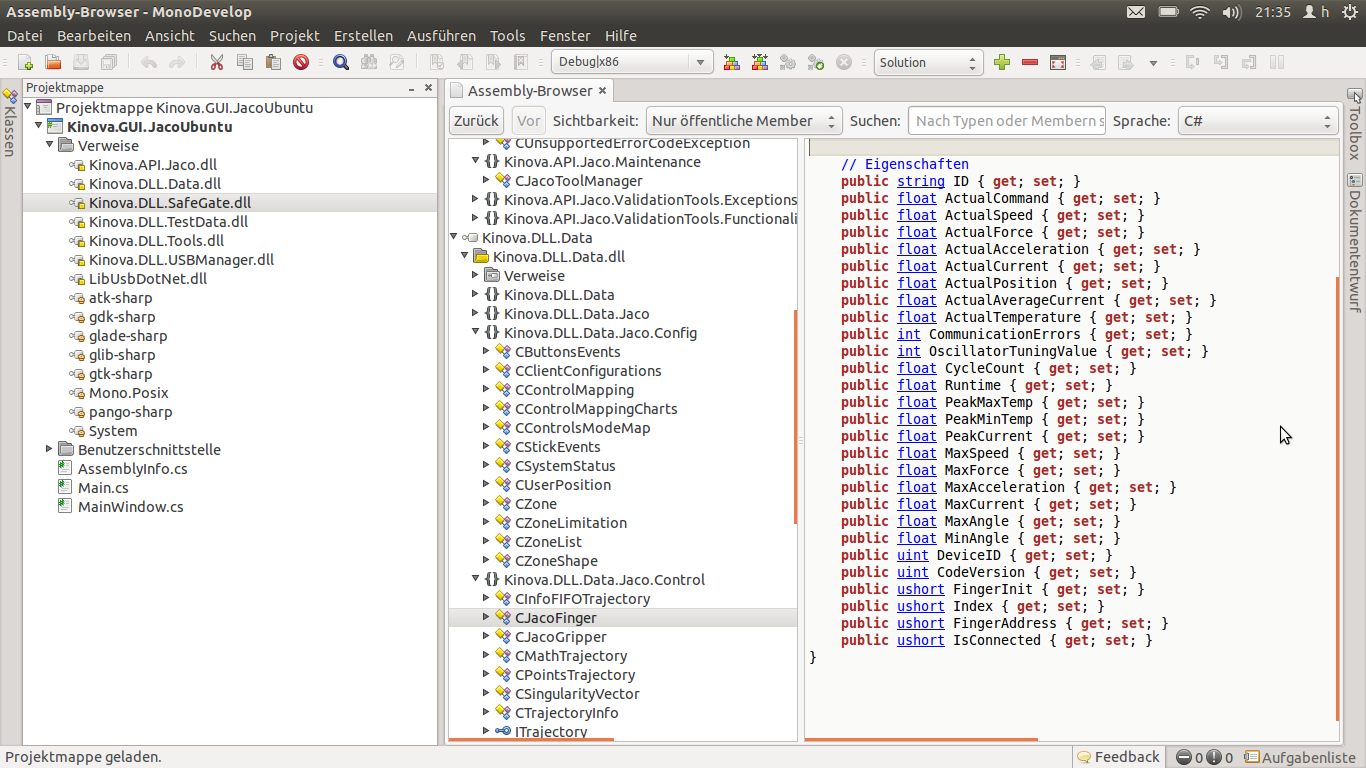
\includegraphics[width=\linewidth]{monodevelop.png}
\end{figure}
}

\frame{\frametitle{Jaco Arm Library}
\begin{itemize} 
\item acceleration, velocity, force, joint temperature,.... 
\item protection zones
\item trajectories
\end{itemize} 
}

\frame{\frametitle{Jaco Arm Library}
\begin{figure}
\centering
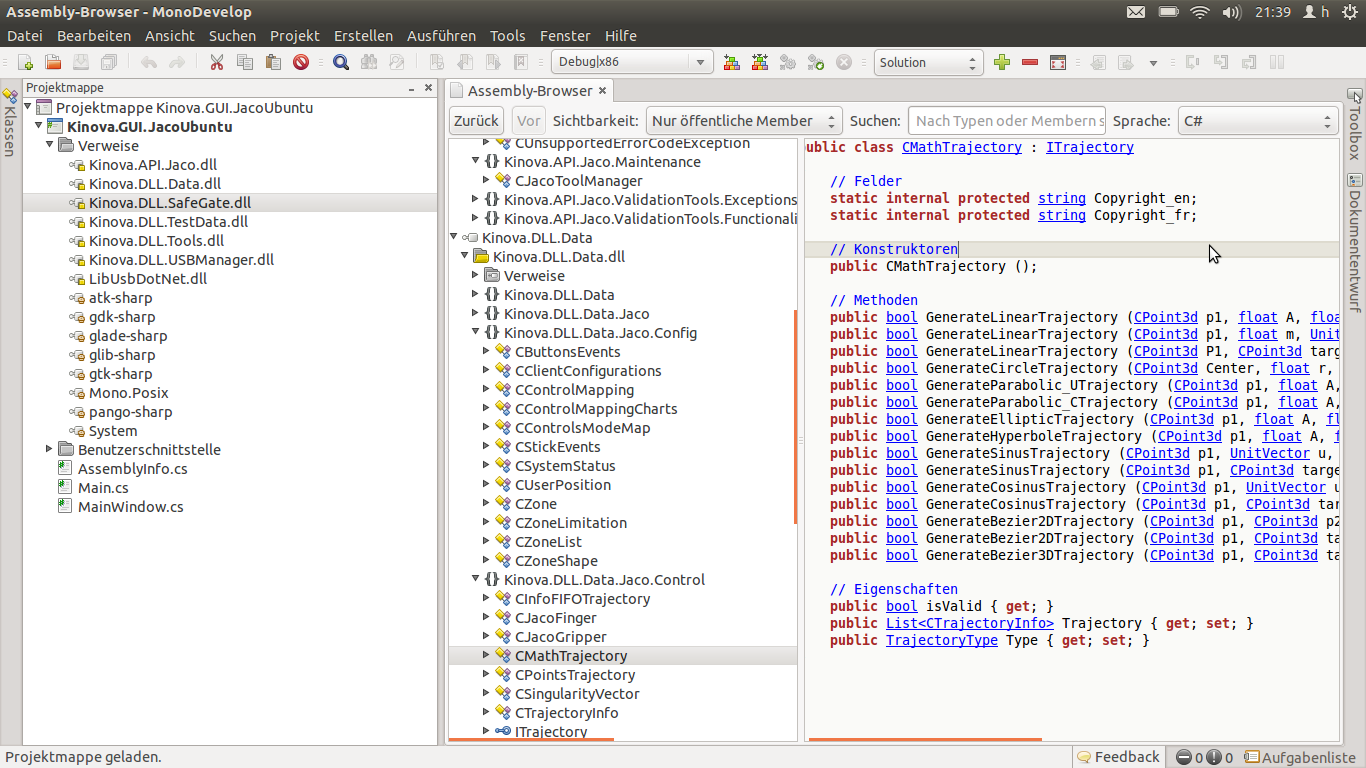
\includegraphics[width=\linewidth]{monodevelop2.png}
\end{figure}
}


\section{Jaco Arm ROS Stack}

\frame{\frametitle{Kinova Jaco Arm ROS Stack}
\begin{itemize} 
\item unofficial ROS stack from Kinova
\item no existing documentation 
\item C\# code into C++ code   
\end{itemize} 
}
 
\frame{\frametitle{Kinova Jaco Arm ROS Stack}
\begin{itemize} 
\item Jaco Node    
\item Jaco State Publisher(\url{robot_state_publisher})
\end{itemize} 
}
  
\frame{\frametitle{\url{Jaco_Node} Subscriber Topics}
\begin{itemize}
\item \url{/jaco_node/cur_goal(geometry_msgs/PoseStamped)}
\item \url{/hand_pose(geometry_msgs/PoseStamped)}
\item \url{/joint_states(sensor_msgs/JointState)}
\end{itemize} 
}

\frame{\frametitle{\url{Jaco_Node} Subscriber Messages}
\begin{figure}[htbp]
			 
		    \begin{minipage}[]{0.4\linewidth}
	 		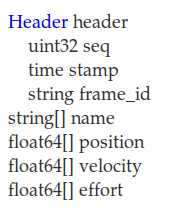
\includegraphics[width=3cm]{jointstate.png}
			\caption{\url{sensor_msgs/JointState}}
		 	\end{minipage}
			\hfill %wichtig, hier keine leerzeile im code
		    \begin{minipage}[]{0.4\linewidth}
	 		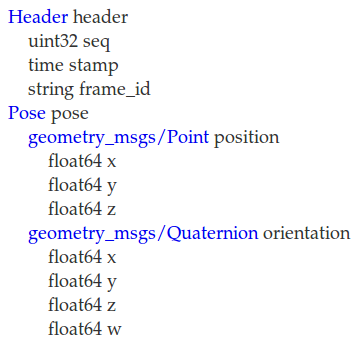
\includegraphics[width=4cm]{geo.png}
			\caption{\url{geometry_msgs/PoseStamped}}
		    \end{minipage}	     
	 \end{figure}
}   				

\frame{\frametitle{\url{Jaco_Node} Publisher Topics/Messages}
\begin{itemize}
\item \url{/hand_goal(geometry_msgs/PoseStamped)}
\item \url{/cmd_abs_finger(jaco_node/FingerPose)}
\item \url{/cmd_abs_joint(jaco_node/JointPose)}
\item \url{/cmd_rel_cart(geometry_msgs/Twist)}
\end{itemize} 
}

\frame{\frametitle{\url{Jaco_Node} Publishers/Subscribers}
\begin{itemize}
\item \url{/.../follow_joint_trajectory/result}
\item \url{/.../follow_joint_trajectory/feedback}
\item \url{/.../follow_joint_trajectory/goal}
\item \url{/.../follow_joint_trajectory/status}
\item \url{/.../follow_joint_trajectory/cancel}
\end{itemize} 
}

\frame{\frametitle{\url{Jaco_Node} Joint Trajectory Messages}
\begin{figure}[htbp]
			 
		    \begin{minipage}[]{0.4\linewidth}
	 		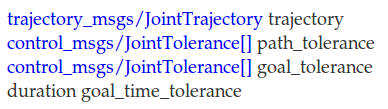
\includegraphics[width=4cm]{goal.png}
			\caption{\url{control_msgs/FollowJointTrajectoryGoal.msg}}
 			\end{minipage}
			%\hfill %wichtig, hier keine leerzeile im code
		    \begin{minipage}[]{0.4\linewidth}
	 		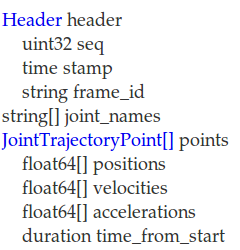
\includegraphics[width=3cm]{jointtrajectory.png}
			\caption{\url{trajectory_msgs/JointTrajectory.msg}}
 		    \end{minipage}	     
	 	
	 \end{figure}
}

\frame{\frametitle{Kinova Jaco Arm ROS Stack}
\begin{itemize} 
\item fixing bugs(open his hand, \url{hand_pose})
\item integrate more functionality
\end{itemize} 
}
 				
\section{Open Motion Planning Library}
\begin{frame}
\frametitle{The Open Motion Planning Library (OMPL)}
  \begin{itemize} 
  \item library of sampling-based motion planning algorithms
  \item integrated in ROS arm navigation stack (used on the PR2)
  \item integrated in (new) MoveIt! project
  \item includes state-of-the-art motion planning algorithms
  \item no collision checking
  \item demo videos at \url{http://ompl.kavrakilab.org/gallery.html}
  \item tutorials on how to integrate OMPL at
  \url{http://www.ros.org/wiki/ompl_ros_interface/Tutorials}
  \end{itemize} 
\end{frame}

\frame{\frametitle{MoveIt! - A Planning Framework}
\begin{itemize} 
\item includes kinematics, dynamics, collision checking, constraints evaluation,
visualization ..
\item centered around planning and execution motion plans for different robots
\item Tools include: specification of motion plans, configuration and debugging
tools, visualization, benchmarking
\item Overview at \url{http://moveit.ros.org}
\end{itemize} 
}

\frame{\frametitle{MoveIt! - A Planning Framework}
\begin{figure}
\centering
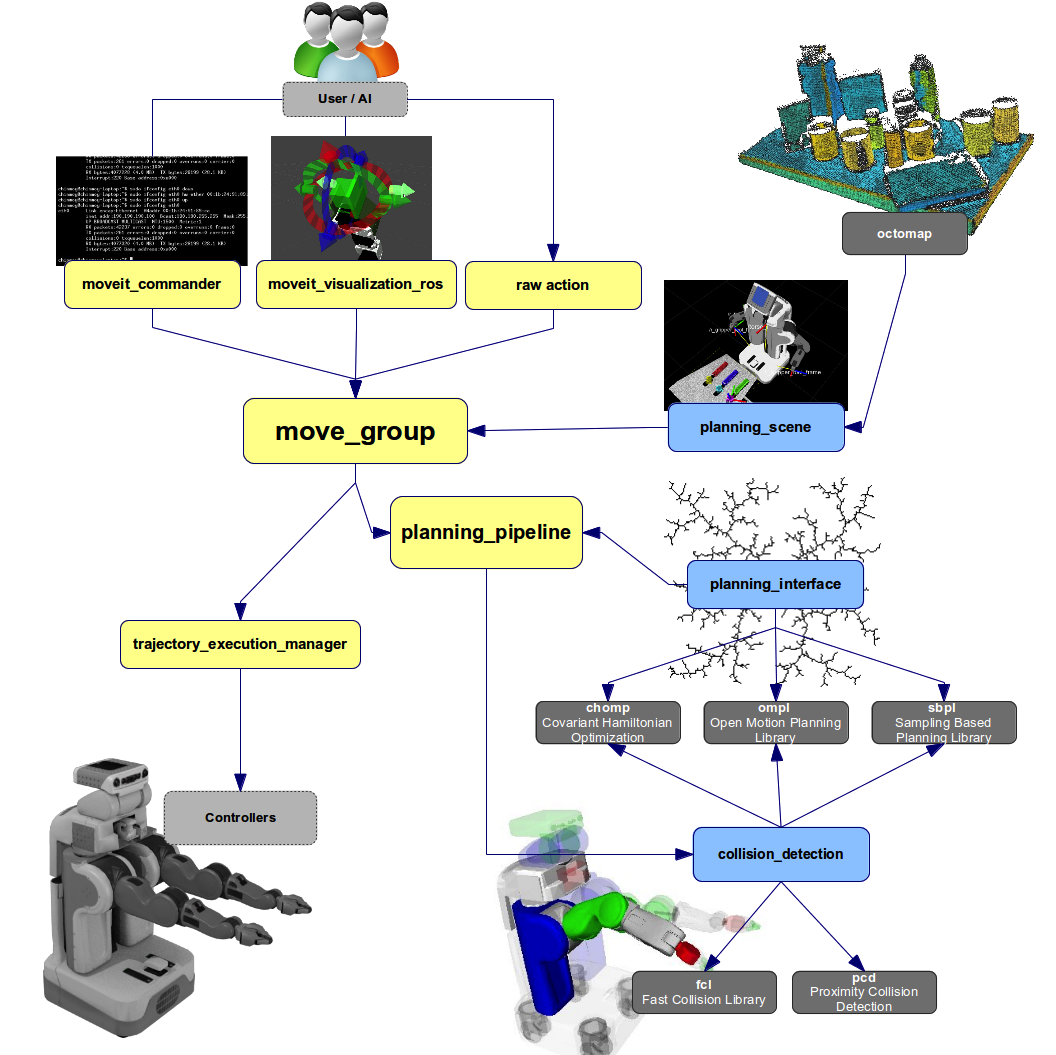
\includegraphics[height=0.85\textheight]{images/moveit_highlevel_cut.png}
\end{figure}

}

\section{Demo}
\frame{\frametitle{Demo}
\begin{figure}
\centering
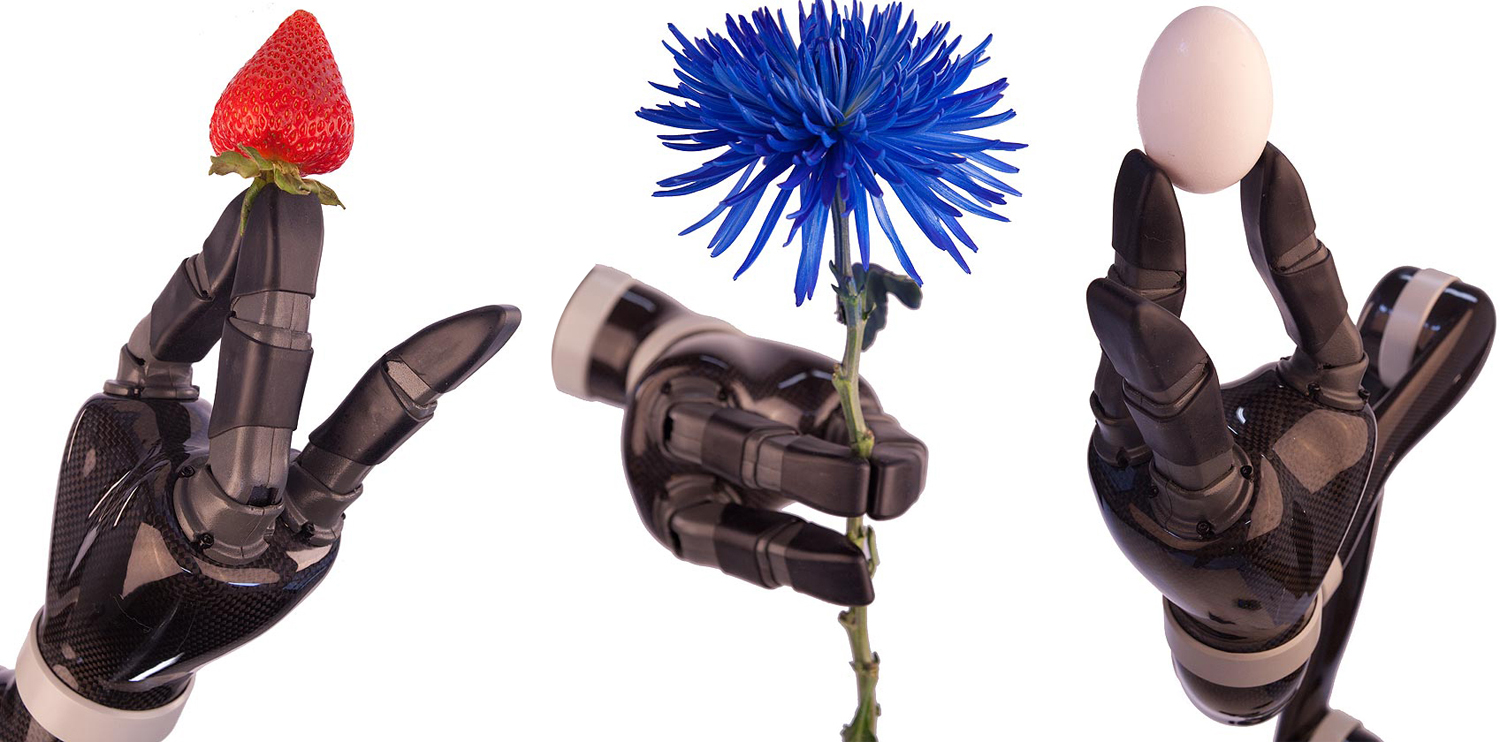
\includegraphics[width=\linewidth]{kinova.jpg}
\end{figure}
}
    
\end{document}
